\documentclass[aspectratio=169,10pt]{beamer}\usetheme{default}\usecolortheme{seahorse}\setbeamertemplate{navigation symbols}{}\setbeamertemplate{footline}[frame number]
\usepackage[T1]{fontenc}\usepackage[utf8]{inputenc}\usepackage{helvet}\usepackage{booktabs,amsmath}
\setbeamertemplate{footline}{\hfill{\tiny\textcolor{red!70!black}{DRAFT for the author\textquoteright{}s review, November 10, 2026}\quad\insertframenumber}\hspace{1em}\vspace{0.4em}}
\title{Weather, daylight, snow and bicycle traffic on rue de Terrebonne}\subtitle{Five count series, August 2024 to November 2026: methods in brief and the main results}\author{Rick Hoge, PhD}\institute{Terrebonne-open-sources}\date{November 10, 2026}
\begin{document}
\begin{frame}\titlepage\end{frame}
\begin{frame}{The question and the sources}
\begin{itemize}
\item How does the number of bicycles counted on rue de Terrebonne vary with temperature, wind chill, rain, snow, daylight and snow loading?
\item Five series, each analysed on its own and never compared in level:
\begin{itemize}\footnotesize
\item \textbf{King Edward} and \textbf{Draper}: the author\textquoteright{}s Telraam camera sensors, bicycles 08:00--16:00 (691 and 509 valid days from August and September 2024)
\item \textbf{Kensington loop}: the borough\textquoteright{}s counter, eastbound, 24 h (284 days, July 27, 2025 to May 10, 2026; hourly release of June 4, 2026)
\item \textbf{BIXI station} Grand Boulevard / de Terrebonne: trips starting or ending, regular season
\item \textbf{City counters}: twelve loop counters elsewhere in Montréal, as a reference
\end{itemize}
\item Weather: Environment and Climate Change Canada, Montréal-Trudeau (daily rain, snowfall, snow on the ground; hourly temperature and wind). Snow loading: the City\textquoteright{}s record for sector CDN-301.
\end{itemize}
\end{frame}
\begin{frame}{The record}
\centering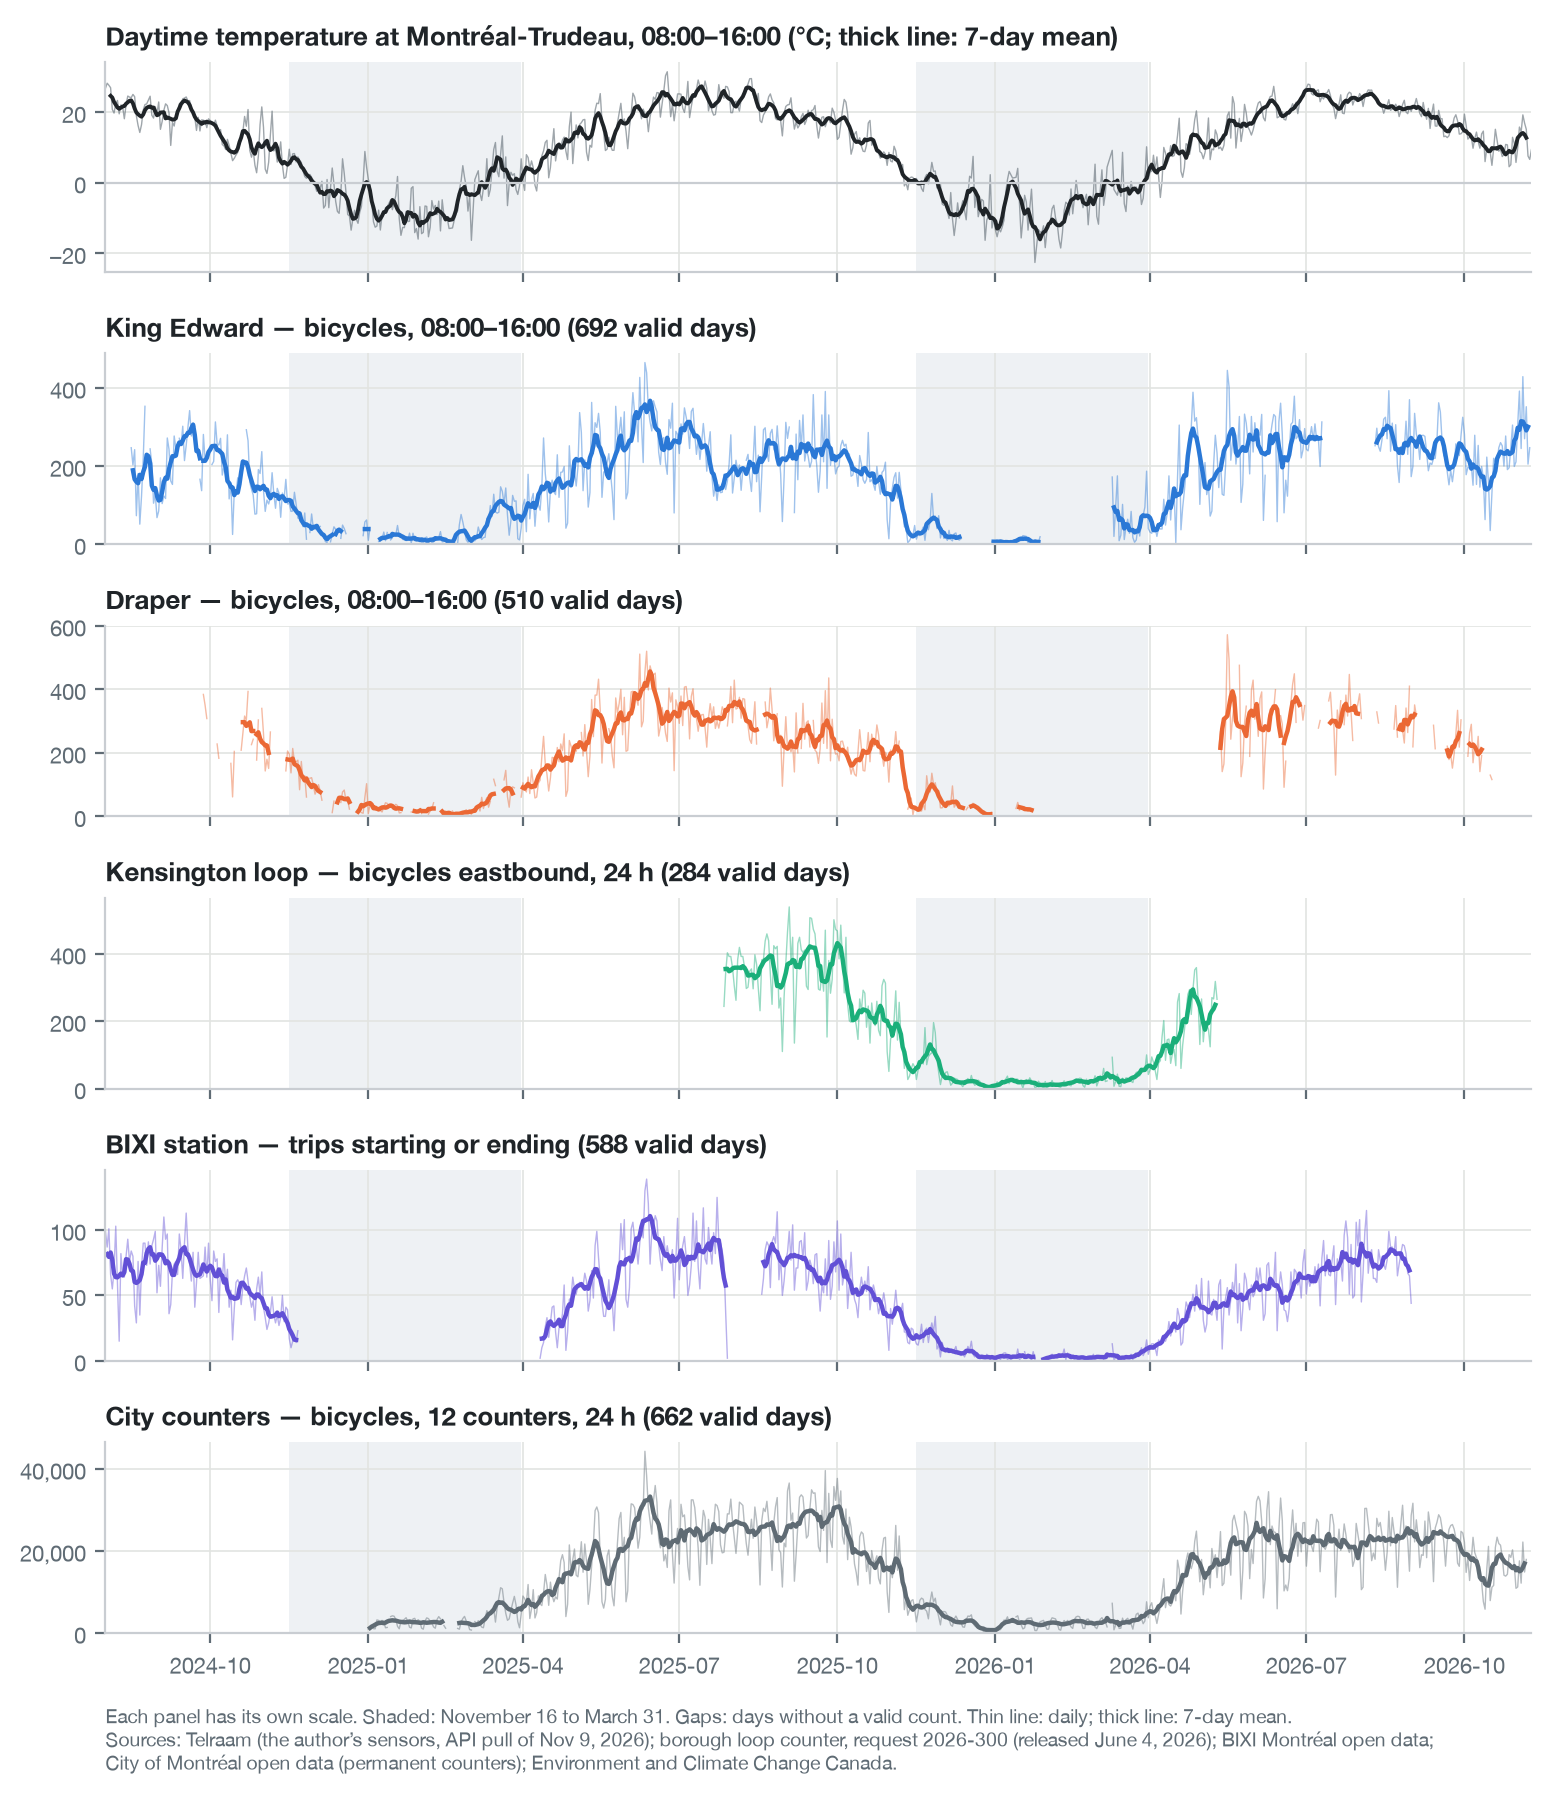
\includegraphics[width=0.55\textwidth,height=0.76\textheight,keepaspectratio]{../derived/figures/overview/overview_en.png}\\[0.2em]{\scriptsize Each panel has its own scale.}
\end{frame}
\begin{frame}{Method (1): what is counted}
\begin{itemize}
\item A Telraam sensor counts \textbf{only in daylight}: about 9 hours in December, 16 in June. Its daily total moves with the length of the day even if riding does not.
\item Every Telraam figure here is the count in a \textbf{fixed window, 08:00--16:00}, daylight all year. The evening peak is left out.
\item Valid day: at least 8 reported hours and 6 hours of uptime, and all eight window hours with uptime of 0.5 or more. Nothing is interpolated.
\item The loop: eastbound channel only (the westbound channel under-counts from about March 1, 2026).
\item BIXI: a day without a trip is absent from the file, not a zero; April 15 to November 15 only in the models.
\end{itemize}
\end{frame}
\begin{frame}{Method (2): the model}
\begin{itemize}
\item One \textbf{negative binomial regression per series}, log link: every effect is a percentage change, so series can be set side by side without comparing levels.
\item Terms: day type, holidays, counting year, time of year (two annual harmonics), daytime temperature, rain and snowfall in classes, snow on the ground, wind, snowfall of the day before.
\item Temperature: a spline, and a line with one change of slope whose position is estimated.
\item Intervals robust to autocorrelation (Newey--West); moving-block bootstrap for the change of slope.
\item Checks: effects re-estimated inside calendar months; each month left out and predicted; wind chill in place of temperature; an hourly model of the loop for darkness.
\end{itemize}
\end{frame}
\begin{frame}{Temperature: the raw relation}
\centering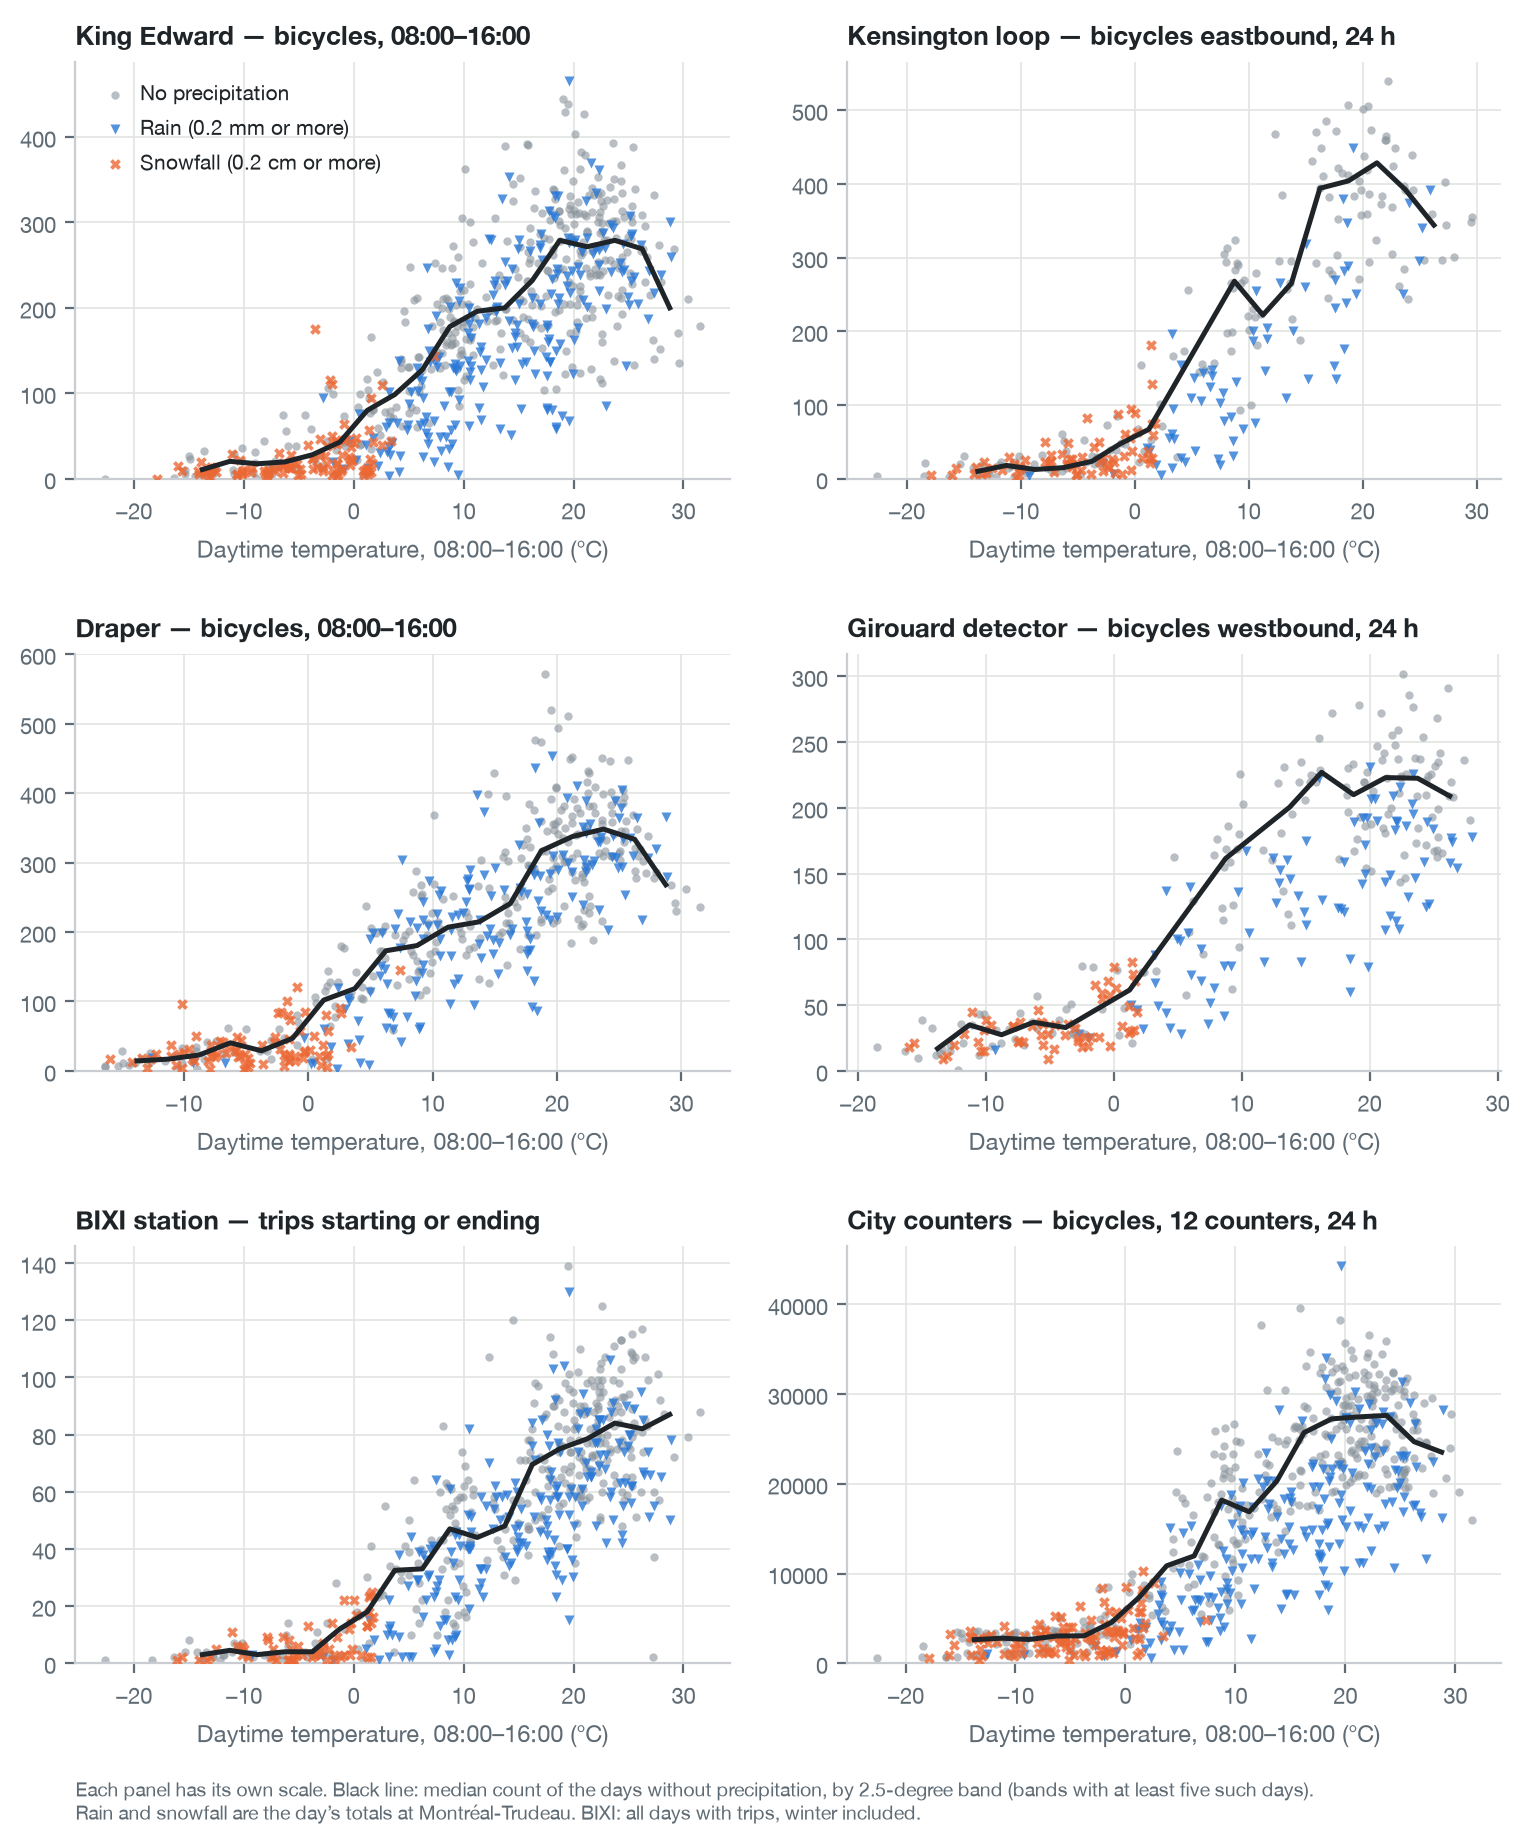
\includegraphics[width=0.62\textwidth,height=0.76\textheight,keepaspectratio]{../derived/figures/temperature-scatter/temperature_scatter_en.png}\\[0.2em]{\scriptsize Each panel has its own scale. Black line: median of the days without precipitation.}
\end{frame}
\begin{frame}{Temperature: the fitted response, relative to 20\,$^\circ$C}
\centering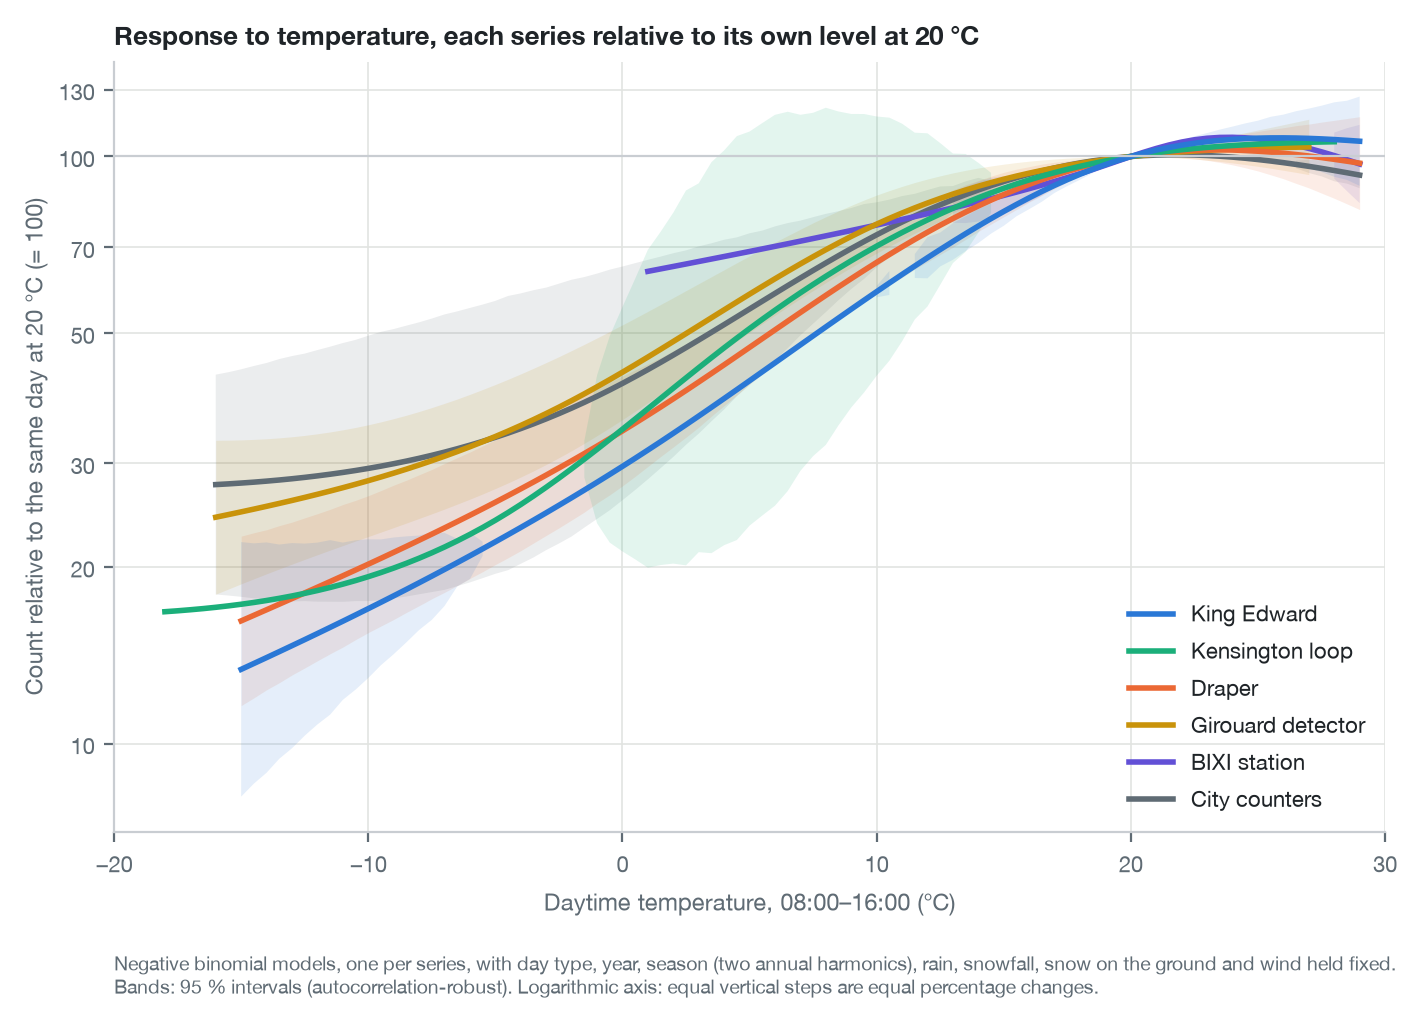
\includegraphics[width=0.66\textwidth,height=0.76\textheight,keepaspectratio]{../derived/figures/temperature-curve/temperature_curve_en.png}\\[0.2em]{\scriptsize Terrebonne series: 5 to 6\,\% more bicycles per degree up to roughly 20\,$^\circ$C; at 0\,$^\circ$C, 30 to 34\,\% of the count at 20\,$^\circ$C; at $-$10\,$^\circ$C, 17 to 20\,\%.}
\end{frame}
\begin{frame}{Temperature: what the fits say}
\begin{itemize}
\item Below roughly 20\,$^\circ$C, each degree goes with 5 to 6\,\% more bicycles on the three Terrebonne series; the same inside calendar months.
\item Above that the count is flat or falls slightly. The position of the bend is poorly determined (intervals of ten degrees or more): the response bends gradually.
\item \textbf{No second change of slope in the cold}: below 0\,$^\circ$C the percentage slope is not distinguishable from the slope between 0 and 20\,$^\circ$C.
\item The $-$1 and $-$5\,$^\circ$C thresholds of the earlier analyses came from fitting straight lines to the counts themselves.
\item Wind chill in place of temperature and wind fits about as well (correlation 0.996); the data cannot separate them.
\end{itemize}
\end{frame}
\begin{frame}{Rain, snow and wind at a given temperature and time of year}
\centering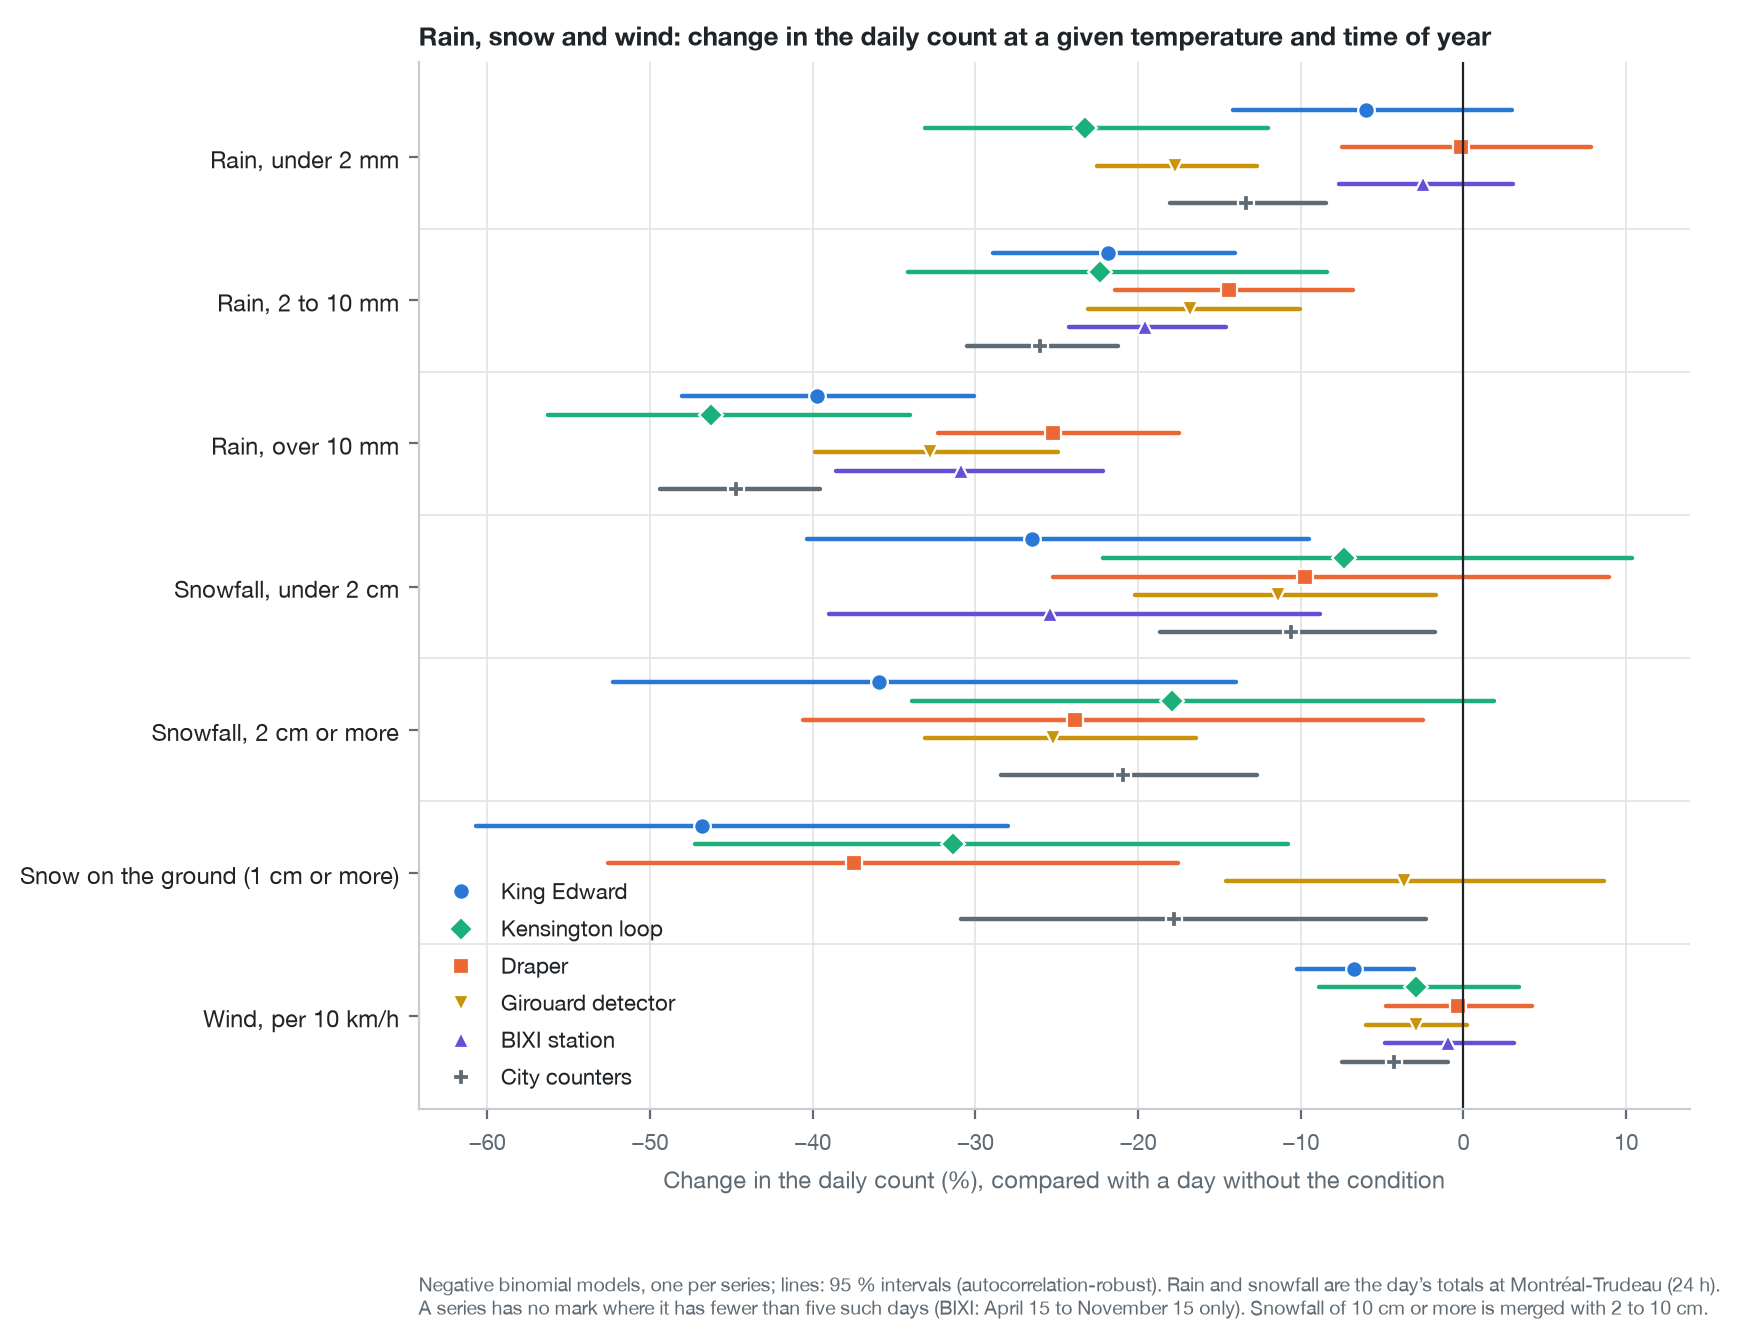
\includegraphics[width=0.66\textwidth,height=0.76\textheight,keepaspectratio]{../derived/figures/effects/effects_en.png}
\end{frame}
\begin{frame}{Season or weather?}
\centering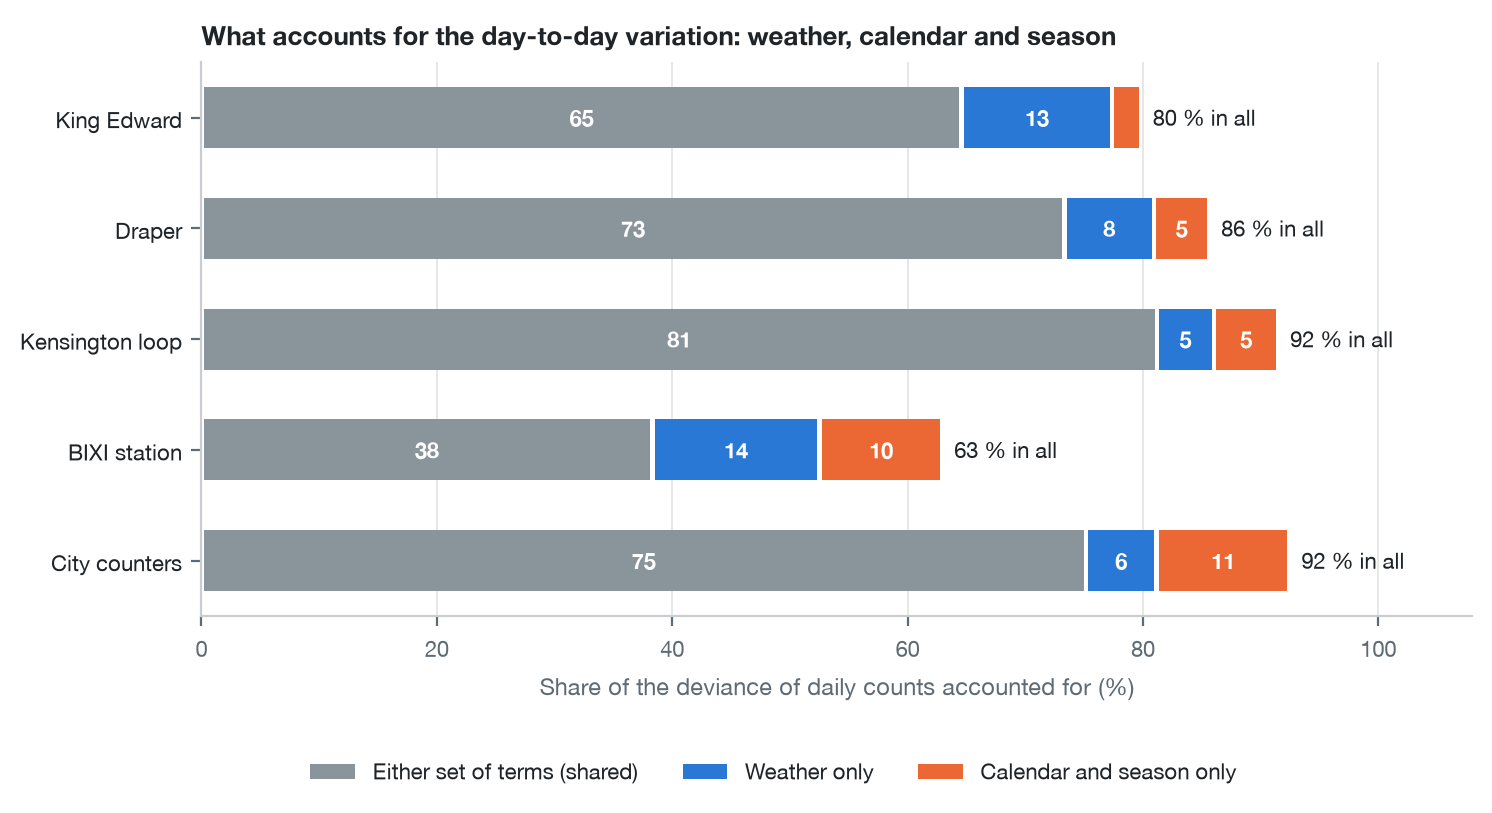
\includegraphics[width=0.74\textwidth,height=0.76\textheight,keepaspectratio]{../derived/figures/season-weather/season_weather_en.png}\\[0.2em]{\scriptsize Most of what the models account for can be credited to either: the record cannot fully separate season from weather. Weather effects estimated inside calendar months are the same.}
\end{frame}
\begin{frame}{Day length: what a daylight-only sensor sees}
\centering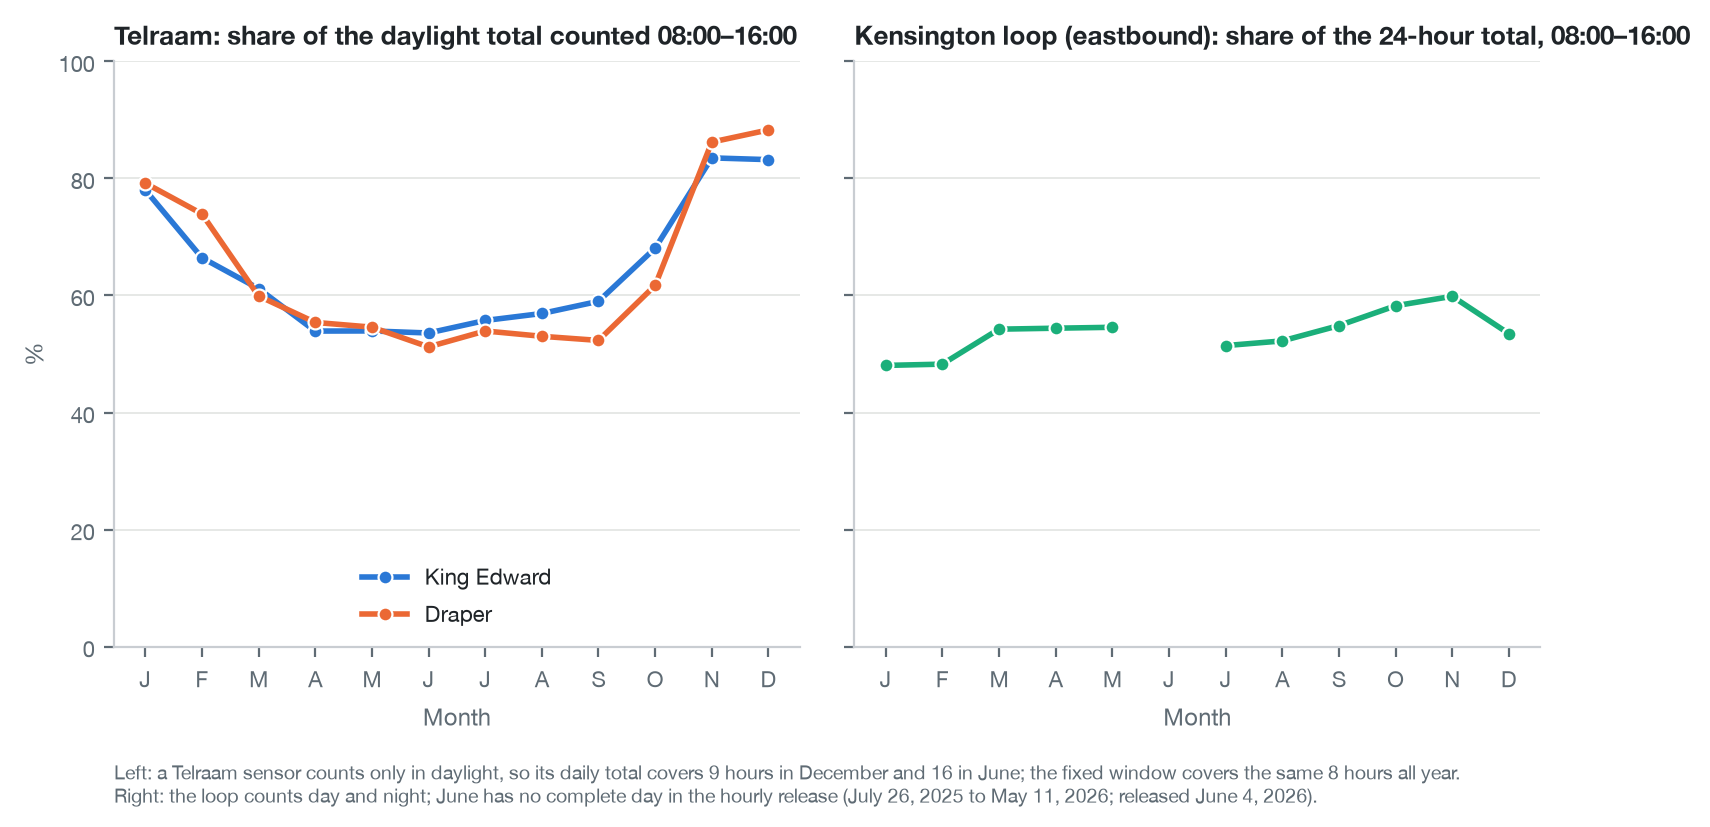
\includegraphics[width=0.84\textwidth,height=0.76\textheight,keepaspectratio]{../derived/figures/daylight/daylight_en.png}\\[0.2em]{\scriptsize On the loop (hourly), the same evening hour carries 27\,\% (19 to 34) fewer bicycles after sunset than before, at the same temperature and in the same month.}
\end{frame}
\begin{frame}{Snowfall and the days after (winter days)}
\centering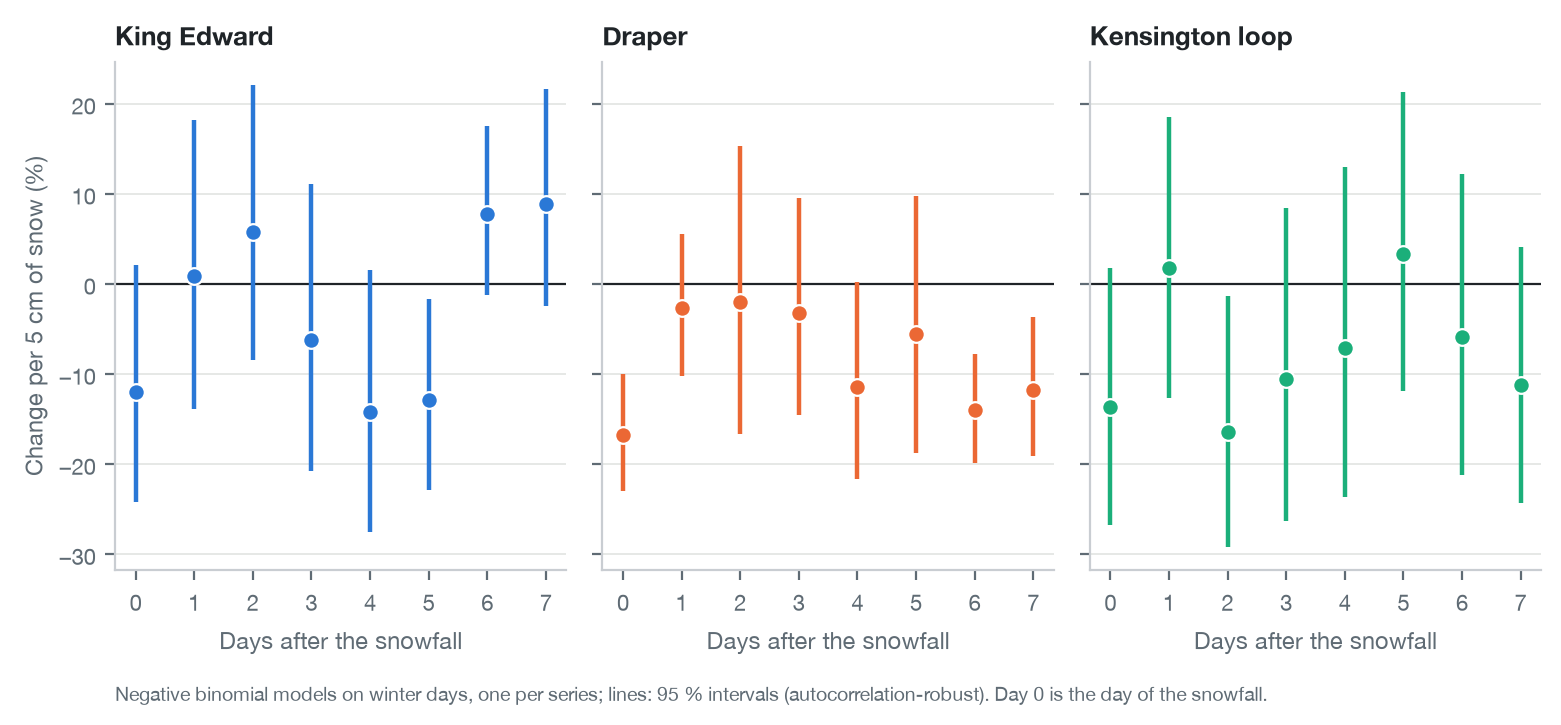
\includegraphics[width=0.9\textwidth,height=0.76\textheight,keepaspectratio]{../derived/figures/snow-lags/snow_lags_en.png}\\[0.2em]{\scriptsize The day of the snowfall shows the clearest reduction; no pattern common to the three series on the following days. Snow on the ground carries part of the after-effect.}
\end{frame}
\begin{frame}{Snow-loading days}
\begin{center}\small\begin{tabular}{lrrl}\toprule
Series & Winter days & Loading days & Change on a loading day (\%)\\\midrule
King Edward & 191 & 44 & $-$4 ($-$29 to +30) \\
Draper & 154 & 37 & $-$21 ($-$48 to +21) \\
Kensington loop & 132 & 36 & +2 ($-$25 to +39) \\
\bottomrule\end{tabular}\end{center}
\begin{itemize}
\item With temperature, snowfall, snow on the ground, rain, wind and day type in the model, loading days are not distinguishable from other winter days.
\item The intervals are wide: they contain no change and a reduction of a quarter or more. The record does not settle the question.
\end{itemize}
\end{frame}
\begin{frame}{How well the models predict}
\begin{center}\small\begin{tabular}{lrrrrr}\toprule
 & & \multicolumn{2}{c}{Median absolute error (\%)} & \multicolumn{2}{c}{$R^2$ (log scale)}\\
Series & Days & Fitted & Month left out & Fitted & Month left out\\\midrule
King Edward & 691 & 22 & 23 & 0.84 & 0.82 \\
Draper & 505 & 19 & 20 & 0.88 & 0.86 \\
Kensington loop & 284 & 20 & 25 & 0.92 & 0.87 \\
BIXI station & 441 & 15 & 17 & 0.59 & 0.50 \\
City counters & 661 & 15 & 18 & 0.94 & 0.93 \\
\bottomrule\end{tabular}\end{center}
Each calendar month in turn is left out and predicted from the rest.
\end{frame}
\begin{frame}{Limits}
\begin{itemize}
\item Telraam figures are 08:00--16:00 counts; never compared in level with the loop.
\item Gaps: King Edward has no valid day in February 2026; Draper none from February to April 2026.
\item The loop: one site, one winter, one direction.
\item Weather at the airport (9 km); precipitation as 24-hour totals; the state of the lane is not observed.
\item Season and weather are confounded; the models describe association in the record, not cause.
\item Year-to-year terms absorb anything that differs between years besides the weather (gaps, sensor position); see the note.
\end{itemize}
\end{frame}
\begin{frame}{Where everything is}
\begin{itemize}
\item Note, tables, figures (English and French) and scripts: \url{https://github.com/OpenMobilityData/Terrebonne-open-sources/tree/main/2026-weather-and-bike-traffic}
\item Sources: Environment and Climate Change Canada; Telraam (the author\textquoteright{}s sensors); borough loop counter (access requests 2026-300, released June 4, 2026, and 2026-581, released October 9, 2026); City of Montréal open data (CC BY 4.0); BIXI Montréal open data.
\end{itemize}
\end{frame}

\end{document}
